\documentclass[11pt]{article}
\usepackage[margin=1in]{geometry}
\usepackage{fancyhdr}
\pagestyle{fancy}
\usepackage{amsmath}
\usepackage{amssymb}
\usepackage[utf8]{inputenc} 
\usepackage{graphicx} 
\usepackage{parskip} 
\usepackage{multirow} 
\usepackage{mathtools}

\DeclarePairedDelimiter\abs{\lvert}{\rvert}%
\DeclarePairedDelimiter\norm{\lVert}{\rVert}%

\makeatletter
\let\oldabs\abs
\def\abs{\@ifstar{\oldabs}{\oldabs*}}

\let\oldnorm\norm
\def\norm{\@ifstar{\oldnorm}{\oldnorm*}}
\makeatother
\usepackage{multicol} 
\usepackage[spanish,es-nodecimaldot]{babel} 
\usepackage{mathtools}
\usepackage{amsfonts}
\usepackage{float}
\usepackage{textcomp}
\usepackage{caption}
\usepackage{subfig}
\usepackage[spanish]{babel}
\usepackage{gensymb}
\def\sen{\mathop{\mbox{\normalfont sen}}\nolimits}

\lhead{Nieto Castellanos Jaime Fabián}
\chead{}
\rhead{Tarea 3. Histogramas}

\begin{document}

Se realizaron histogramas para los PMT F14A y H13C. En la fig.\ \ref{fig:LogScale} se muestran los histogramas en escala logarítmica, en todo el rango de valores y con 5,000 bins. En la fig.\ \ref{fig:NormScale} se muestran los histogramas en escala lineal, en el rango de 0 a 10 y con 500 bins. La selección de calidad de los datos sólo fue realizada revisando si la variable FLAG era igual a cero o no.

\begin{figure}[H]
\centering
\subfloat[\centering]{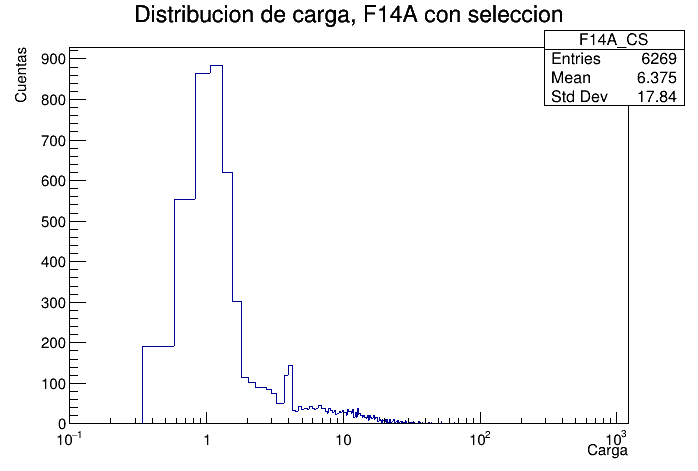
\includegraphics[width=0.5\textwidth]{../F14A_CSLog.png}}
\subfloat[]{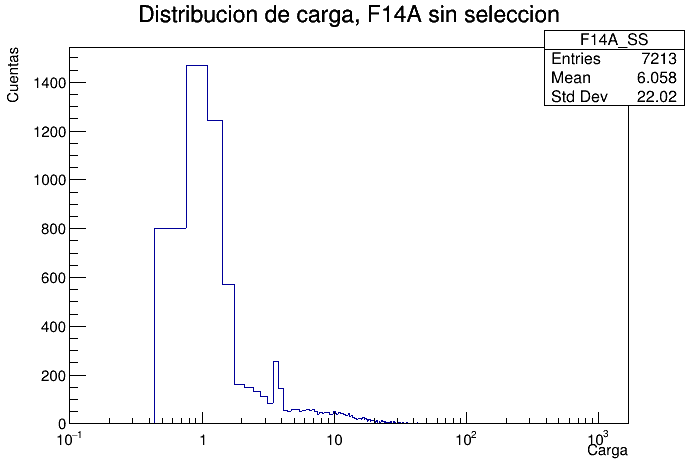
\includegraphics[width=0.5\textwidth]{../F14A_SSLog.png}}

\subfloat[\centering ]{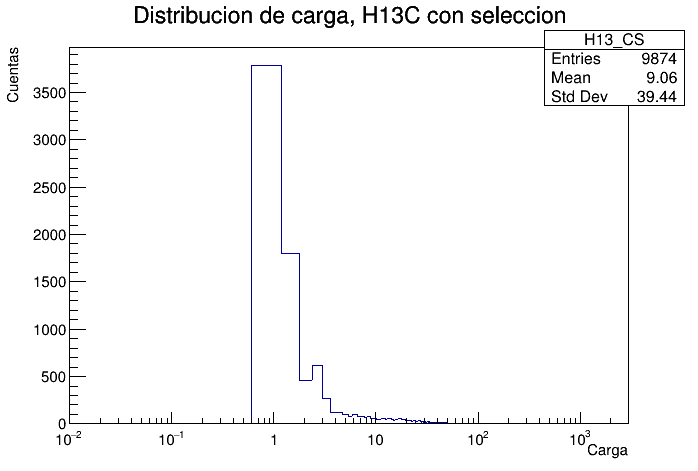
\includegraphics[width=0.5\textwidth]{../H13C_CSLog.png}}
\subfloat[\centering ]{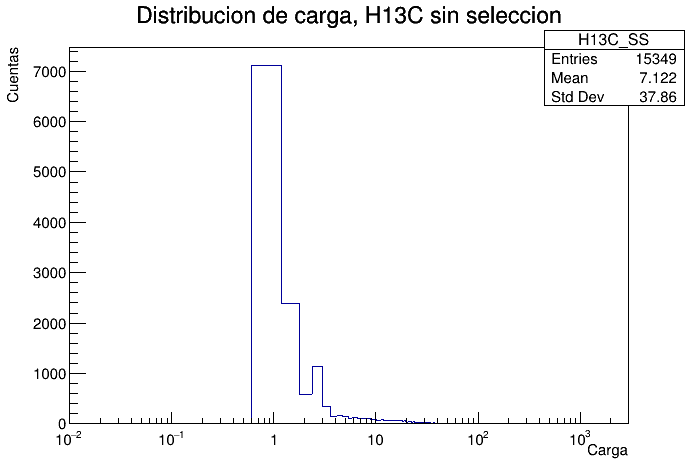
\includegraphics[width=0.5\textwidth]{../H13C_SSLog.png}}
\caption{Se usaron 5,000 bins y escala logarítmica sobre todo el rango de valores de la carga.}
\label{fig:LogScale}
\end{figure}




\begin{figure}[H]
\centering
\subfloat[\centering]{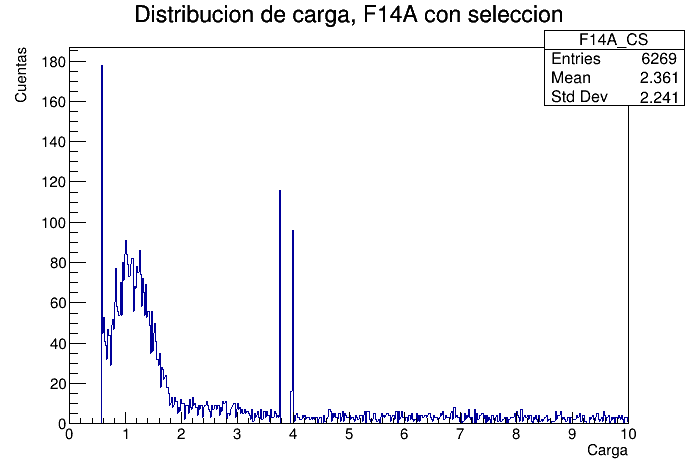
\includegraphics[width=0.5\textwidth]{../F14A_CS.png}}
\subfloat[]{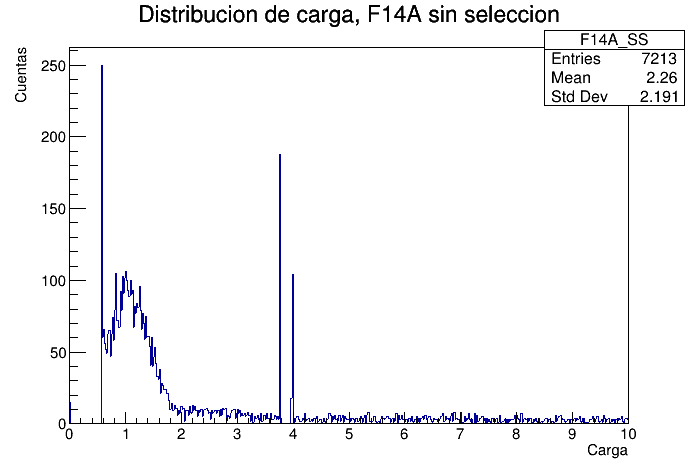
\includegraphics[width=0.5\textwidth]{../F14A_SS.png}}

\subfloat[\centering ]{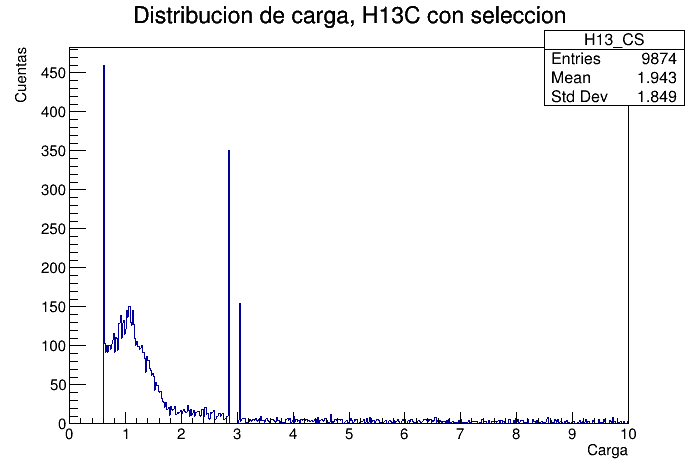
\includegraphics[width=0.5\textwidth]{../H13C_CS.png}}
\subfloat[\centering ]{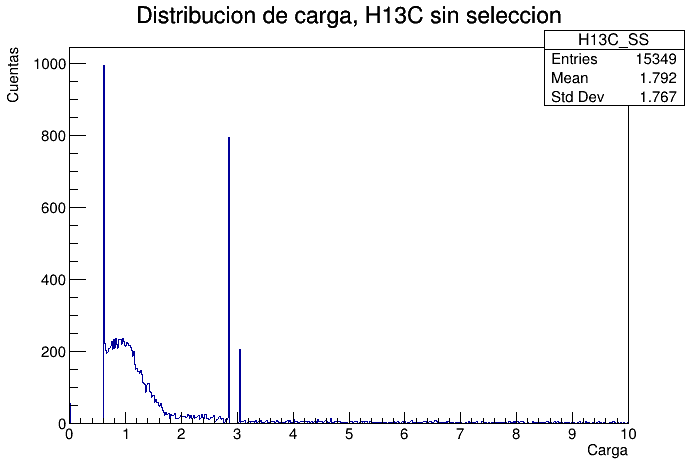
\includegraphics[width=0.5\textwidth]{../H13C_SS.png}}
\caption{Se usaron 500 bins y escala lineal, graficando en el intervalo [0,10] en el eje $x$.}
\label{fig:NormScale}
\end{figure}

En el caso del fotomultiplicador F14A, se observa que hay tres picos, uno en 0.5 PEs y otros dos cerca 3.9 PEs y 4 PEs. Esto se aprecia tanto en los histogramas con selección como sin selección. En el histograma con selección observamos un menor número de cuentas, lo cual es lógico considerando que corresponde a un filtro de los datos totales. 

De forma similar, los histogramas correspondientes al PMT H13C presentan tres picos, uno cerca de 0.5 PEs y otros dos en la cercanía de 3 PEs. Se observa que en general, hay más registro de eventos para el fotomultiplicador H13C que para el F14A. También, en el H13C pareciera que se forma otro pico al hacer la selección de calidad.


\end{document}